\documentclass[titlepage]{article}
\usepackage[utf8]{inputenc}
\usepackage[french]{babel}
\usepackage[margin=1in]{geometry}
\usepackage[T1]{fontenc}
\usepackage[colorlinks=true,linkcolor=teal]{hyperref}
\usepackage{amssymb,amsmath,minted,float,graphicx,textcomp,systeme,listings,physics,lmodern,mathtools,ifthen,esvect,hyperref,fancyhdr,lastpage,marginnote,chngcntr,fancyvrb,subcaption}
\DeclareMathOperator{\e}{e}
\def\mathbi#1{\textbf{\em #1}}

\setlength\parindent{0pt}

%%%%%%%%%%%% PARAMETRES
\newcommand{\UE}{Stage}
\newcommand{\type}{Résultats}%TD-TP-COURS
\newcommand{\nb}{0}%nb 
\newcommand{\sbt}{Reconstruction dynamique d'images radioastronomiques}%soustitre
\author{Gabriel ROBERT-DAUTUN}
\date{2022}

% mise en page (header, compteur, fancy)
\pagestyle{fancy}
\lhead{\UE\, - \type\ifthenelse{\nb > 0}{\nb}{}}
\rfoot{\thepage /\pageref{LastPage}}
\lfoot{}
\cfoot{}
\renewcommand{\footrulewidth}{0.4pt}

%reset compteur section par partie
\counterwithin*{section}{part}

% permet notes + simples en marge à gauche (ig compteur de question)
\reversemarginpar
\newcommand{\mgn}[1]{\marginnote{#1}}

%sinon warning mdr
\setlength{\headheight}{13.07225pt}

%compteur questions
\newcounter{question}
\setcounter{question}{1}
\newcounter{subq}
\setcounter{subq}{1}

\newcommand{\rsubq}{\setcounter{subq}{1}}
\newcommand{\question}{\mgn{\thequestion .}\stepcounter{question}\rsubq}
\newcommand{\rstq}{\setcounter{question}{1}\rsubq}
\newcommand{\skipq}[1]{\addtocounter{question}{#1}\rsubq}
\newcommand{\subq}{\noindent\alph{subq})\stepcounter{subq}} %a modifier pour mettre dans le margin

\title{%
	\UE\, - \type\ifthenelse{\nb > 0}{\nb}{} \\
	\large \sbt}

\begin{document}
	
	\begin{figure}
		\centering
		
\includegraphics[width=0.7\linewidth]{logo.PNG}
		\label{fig:logo}
	\end{figure}
	\maketitle
	
	\newpage
	\tableofcontents
	
	\newpage
	\section{Robustesse et performances}
	\subsection{Erreur sur l'image de départ}
	On introduit une erreur gaussienne sur l'image $X_0$. On observe que le fonctionnement du Kalman est bien celui attendu dans ce cas là : l'erreur dans l'image se réduit petit a petit.
	
	\begin{figure}[H]
		\centering
		\includegraphics[width=0.9\linewidth]{Perfs/Illustration.JPG}
		\caption{En haut : images réelles utilisées pour générer les données. En bas : images reconstruites. Titres : PSNR}
	\end{figure}

	On utilise une transformation de rotation de l'image de 90°. On remarque grâce au PSNR que les images reconstruites s'approchent des images réelles, mais pas parfaitement car le filtre prend en compte l'historique. Une erreur dans une image va donc se diffuser aux images suivantes (précédentes si backwards). On observe la convergence de reconstruction :
	
	\begin{figure}[H]
		\centering
		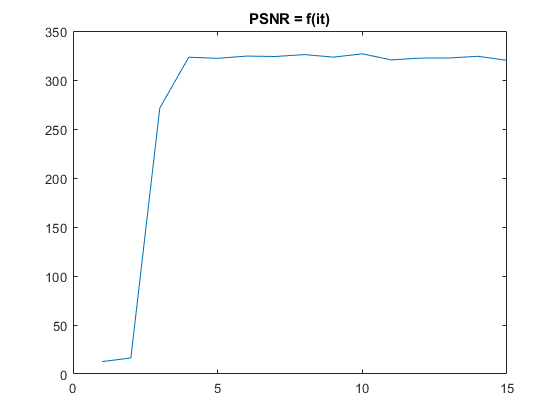
\includegraphics[width=0.9\linewidth]{Perfs/conv02.png}
		\caption{Evolution psnr en fonction du nombre d'itérations}
	\end{figure}

	On converge en 4 itérations au plus a chaque essai : les erreurs gaussienne d'amplitude 0.2 se diffusent sur 4 itérations environ.
	Vérifié pour des amplitude de 0.1 a 1. Pour des amplitudes plus grandes (5 donc SNR=0.1) parfois 5 itérations sont nécessaires
	
\end{document}

\begin{figure}[H]
	\centering
	\includegraphics[width=0.7\linewidth]{}
	\caption{}
\end{figure}

\begin{figure}[H]
	\centering
	\begin{subfigure}{.5\textwidth}
		\centering
		\includegraphics[width=.4\linewidth]{image1}
		\caption{}
	\end{subfigure}%
	\begin{subfigure}{.5\textwidth}
		\centering
		\includegraphics[width=.4\linewidth]{image2}
		\caption{}
	\end{subfigure}
	\caption{}
\end{figure}
